\documentclass[conference, onecolumn]{IEEEtran}

\usepackage{algorithm}
\usepackage{algorithmic}
\usepackage{amsmath}
\usepackage{amssymb}
\usepackage{amsfonts}
\usepackage{siunitx}
\usepackage{standalone}
\usepackage{tikz}
\usetikzlibrary{matrix,backgrounds,calc,shapes,arrows,arrows.meta,fit,positioning}
\usetikzlibrary{chains,shapes.multipart}

\usepackage{pgfplots, pgfplotstable}
\usepgfplotslibrary{units}
\usepackage{xcolor}
\usepackage{xspace}
\usepackage{listings}
\usepackage{color}
\usepackage{framed}

\definecolor{dkgreen}{rgb}{0,0.6,0}
\definecolor{gray}{rgb}{0.5,0.5,0.5}
\definecolor{mauve}{rgb}{0.58,0,0.82}

\lstset{frame=tb,
language=C,
aboveskip=3mm,
belowskip=3mm,
showstringspaces=false,
basicstyle={\small\ttfamily},
numbers=none,
numberstyle=\tiny\color{gray},
keywordstyle=\color{blue},
commentstyle=\color{dkgreen},
stringstyle=\color{mauve},
breaklines=true,
breakatwhitespace=true,
tabsize=4
}

%columns=flexible,
\hyphenation{op-tical net-works semi-conduc-tor}
\newcommand{\ts}{\textsuperscript\xspace}
\newcommand{\tst}{\textsuperscript{3}\xspace}


\begin{document}

\title{Micropp: Reference Manual}

%\author{\IEEEauthorblockN{
%	Guido Giuntoli\IEEEauthorrefmark{1}\IEEEauthorrefmark{3},
%	Jimmy Aguilar\IEEEauthorrefmark{1}\IEEEauthorrefmark{4}
%	Judica\"el Grasset\IEEEauthorrefmark{2}\IEEEauthorrefmark{5}}
%\IEEEauthorblockA{\IEEEauthorrefmark{1}Barcelona Supercomputing Center, Spain}
%\IEEEauthorblockA{\IEEEauthorrefmark{2}STFC Daresbury Laboratory, UK}
%\IEEEauthorblockA{\IEEEauthorrefmark{3}guido.giuntoli@bsc.es}
%\IEEEauthorblockA{\IEEEauthorrefmark{4}jimmy.aguilar@bsc.es}
%\IEEEauthorblockA{\IEEEauthorrefmark{5}judicael.grasset@stfc.ac.uk}}

\author{
Guido Giuntoli (gagiuntoli@gmail.com) \\
Jimmy Aguilar (spacibba@aol.com) \\
Judica\"el Grasset (judicael.grasset@stfc.ac.uk)
}

\maketitle

% no keywords

\IEEEpeerreviewmaketitle

\section{Introduction}
% no \IEEEPARstart

\hfill August 26, 2015

\begin{figure}
	\centering
	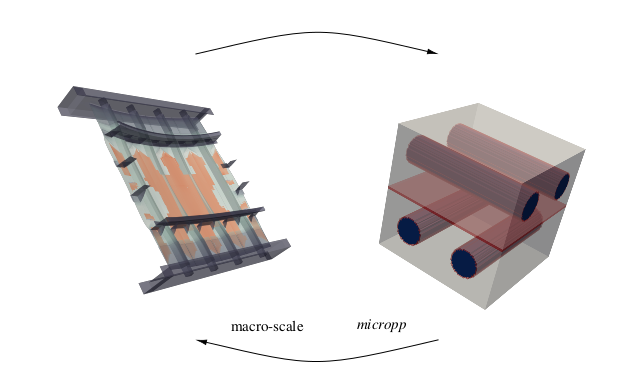
\includegraphics[width=0.95\linewidth]{figures/coupling-micropp-macro.png}
	\caption{\label{fig:disp}
		Coupling between a macro-scale solid mechanics code and Micropp to simulate a composite material
		problem.
	}
\end{figure}

\input{governing_equations_and_fe.tex}

\section{Implementation}

The Voigt convention used here is the same as in Ref.~\cite{simo}.

\begin{equation}
\epsilon = \left[\epsilon_{12} \quad \epsilon_{22} \quad \epsilon_{33} \quad \epsilon_{12} \quad \epsilon_{13} \quad \epsilon_{23} \right]^T
\end{equation}

\section{Geometries}

\section{Material Models}

\subsubsection{Plasticity Model}

MicroPP has a J2 plasticity model with isotropic hardening.

\begin {equation}
\left\{
\begin{array}{ll}
\epsilon_{n+1}^{e,\text{trial}} = \epsilon_{n+1} - \epsilon_{n}^{p} \\[5pt]
\sigma_{n+1}^{\text{trial}} = \mathrm{C} : \epsilon_{n+1}^{e,\text{trial}} \\[5pt]
\mathbf{q}_{n+1}^{\text{trial}} = \mathbf{q}_{n} \\[5pt]
f_{n+1}^{\text{trial}} = f (\sigma_{n+1}^{\text{trial}}, \mathbf{q}_{n+1}^{\text{trial}})\\
\end{array}
\right.
\end {equation}

\begin {equation}
\left\{
\begin{array}{ll}
\epsilon_{n+1}^{p} = \epsilon_{n}^{p} - \Delta \gamma  \mathbf{n}_{n+1} \\[5pt]
\alpha_{n+1} = \alpha_{n} + \sqrt{\frac{2}{3}} \Delta \gamma
\end{array}
\right.
\end {equation}

\begin {equation}
s_{n+1}^{\text{trial}} = s_{n+1} + 2 \mu e_{n+1}
\end {equation}

\begin {equation}
\mathbf{n}_{n+1} = \frac{s_{n+1}^{\text{trial}}}{|| s_{n+1}^{\text{trial}} ||}
\end {equation}

\begin {equation}
f_{n+1}^{\text{trial}} = || s_{n+1}^{\text{trial}} || - \sqrt{\frac{2}{3}} (\sigma_{Y} + K_{a} \alpha_{n} )
\end {equation}

\begin {equation}
\Delta \gamma = \frac{f_{n+1}^{\text{trial}}}{2\mu(1+K_{a})}
\end {equation}

1. Compute trial elastic stress
\begin {equation}
\left\{
\begin{array}{ll}
e_{n+1} = \epsilon_{n+1} - \frac{1}{3} \text{tr}( \epsilon_{n+1} ) \\[5pt]
s_{n+1}^{\text{trial}} = 2\mu( e_{n+1} - e_{n+1}^{p} ) \\[5pt]
\end{array}
\right.
\end {equation}

2. Check yield condition

\begin {equation}
f_{n+1}^{\text{trial}} = || s_{n+1}^{\text{trial}} || - \sqrt{\frac{2}{3}} (\sigma_{Y} + K_{a} \alpha_{n} )
\end {equation}

3. If $f_{n+1}^{\text{trial}} < 0$ then set
\begin {equation}
(\cdot)_{n+1} = (\cdot)_{n+1}^{\text{trial}} \text{ and exit.}
\end {equation}

\begin {equation}
\Delta \gamma = \frac{f_{n+1}^{\text{trial}}}{2\mu(1+K_{a})}
\end {equation}

4. Compute
\begin {equation}
\mathbf{n}_{n+1} = \frac{s_{n+1}^{\text{trial}}}{|| s_{n+1}^{\text{trial}} ||}
\end {equation}

\begin {equation}
\Delta \gamma = \frac{f_{n+1}^{\text{trial}}}{2\mu(1+K_{a})}
\end {equation}

5. Update variables
\begin {equation}
\left\{
\begin{array}{ll}
\epsilon_{n+1}^{p} = \epsilon_{n}^{p} - \Delta \gamma  \mathbf{n}_{n+1} \\[5pt]
\alpha_{n+1} = \alpha_{n} + \sqrt{\frac{2}{3}} \Delta \gamma \\[5pt]
\sigma_{n+1} = k \, \text{tr} (\epsilon_{n+1}) + s_{n+1}^{\text{trial}} - 2 \mu \Delta \gamma \mathbf{n}_{n+1}
\end{array}
\right.
\end {equation}

\begin{algorithm}
\caption{Algorithm caption}
\label{alg:algorithm-label}
\begin{algorithmic}
 \STATE $ \epsilon^{0} = \epsilon $
 \STATE $ \sigma^{0} = g(\epsilon^{0})$
 \FOR {$i=1\dots6$}
     \STATE $ \epsilon^{*} = \epsilon $
     \STATE $ \epsilon^{*}(i) = \epsilon^{*}(i) + \delta\epsilon $
     \STATE $ \sigma^{*} = g(\epsilon^{*})$
     \STATE $ \mathrm{C} (i, :) = ( \sigma^* - \sigma^0 ) / \delta\epsilon $
 \ENDFOR
\end{algorithmic}
\end{algorithm}

\section{Coding Style}

The compilation process is based on \texttt{CMake}



\section{Coding Style}

The coding style should be follow in all .cpp, .hpp, and .f95 files that are present in the code.

\subsection{License}

All source files should have the GPL License header with the corresponding contributors.

\begin{lstlisting}

/*
 *  This source code is part of MicroPP: a finite element library
 *  to solve microstructural problems for composite materials.
 *
 *  Copyright (C) - 2018 - Jimmy Aguilar Mena <kratsbinovish@gmail.com>
 *                         Guido Giuntoli <gagiuntoli@gmail.com>
 *
 *  This program is free software: you can redistribute it and/or modify
 *  it under the terms of the GNU General Public License as published by
 *  the Free Software Foundation, either version 3 of the License, or
 *  (at your option) any later version.
 *
 *  This program is distributed in the hope that it will be useful,
 *  but WITHOUT ANY WARRANTY; without even the implied warranty of
 *  MERCHANTABILITY or FITNESS FOR A PARTICULAR PURPOSE.  See the
 *  GNU General Public License for more details.
 *
 *  You should have received a copy of the GNU General Public License
 *  along with this program.  If not, see <https://www.gnu.org/licenses/>.
 */

\end{lstlisting}

\subsection{Functions Definitions}

Most of the functions in the code are templates. This was done to separate 2D from 3D cases and to produce a more readable code. Functions' arguments can have the \verb const at the beginning but we don't we try to not use it in does cases where it is obvious that the two arguments are not going to be modified. In some cases it it useful if it is applied to pointers like {\verb#int const * a#}.

\begin{lstlisting}

template <int tdim>
int micropp<tdim>::calc_average(const int gp,
                                 double * array
				 int n)
{
	INST_START; /* This is to instrument this function */

	int average = gp + 2.3 / 9.;
	for(int i = 0; i < n / 2; ++i)
		array[i] = average;
	return average;
}
\end{lstlisting}

\subsection{Control Flow Statements}


The \verb if  statements should be written:

\begin{lstlisting}

if(a == 3 && b < 4.) {
    calc_average(a, array, n);
} else if(k % 3 = 2) {
    calc_average(c, array, n);
}

if(calc_average(c, array, n))
    exit(0);

\end{lstlisting}

The \verb for  statements should be written:

\begin{lstlisting}

for(int i = 0; i < n; ++i) {
    a += array[i] + 9.4;
}

for(int i = 0; i < n; ++i)
    for(int j = 0; j < n; ++j)
        array[i * n + j] = A[i][j];

\end{lstlisting}



\section{Benchmarks}


\subsection{\texttt{benchmarks-sol-ass}}

This benchmark is intended to measure the computing times of the assembly of the Residue vector ($\times2$) and the
Jacobian matrix and the solver (CGPD).

Basically the benchmark executes a tipical Newton-Raphson iteration:

\begin{lstlisting}
	double norm = assembly_rhs_acc(u, nullptr, b);

#ifdef _OPENACC
	assembly_mat_acc(&A, u, nullptr);
#else
	assembly_mat(&A, u, nullptr);
#endif

#ifdef _OPENACC
	int cg_its = ell_solve_cgpd_acc(&A, b, du, &cg_err);
#else
	int cg_its = ell_solve_cgpd(&A, b, du, &cg_err);
#endif

	for (int i = 0; i < nn * dim; ++i)
		u[i] += du[i];

	norm = assembly_rhs_acc(u, nullptr, b);
\end{lstlisting}

\begin{figure}[!htbp]
	\centering
	\begin{tikzpicture}[]
		\pgfplotsset{every tick label/.append style={font=\small}}
		\pgfplotstableread{data/benchmark-sol-ass-macintosh.dat}{\times}
		\begin{axis}[
%			grid=major,
%			y unit=s,
%			legend pos=north west,
%			legend cell align={left},
%			ylabel=Computing Time,
%			xlabel=Micro-resolution,
%			x unit=\# Elements,
%			ymin = 0,
%			ymax = 600,
%			xtick = {0,20,40,60,80,100},
%			xticklabels = {0,20\tst,40\tst,60\tst,80\tst,100\tst},
%			ytick = {0,200,400,600,800},
			]
			\addplot [color=blue,mark=*,line width = 0.5mm] table [x index={0}, y index={1}] {\times};
			\addplot [color=green,mark=*,line width = 0.5mm] table [x index={0}, y index={2}] {\times};
%				%{\times} [yshift=9pt] 
%				%node[pos=0.0,yshift=10pt] {36\%}
%				%node[pos=0.105,yshift=11pt] {68\%}
%				%node[pos=1.0] {79\%};
%			%\addplot [color=blue ,mark=*,line width = 0.5mm]  table [x={n1}, y expr=\thisrowno{2}*1.0e-6]
%				%{\times} [yshift=9pt] 
%				%node[pos=0.0] {64\%}
%				%node[pos=0.253,yshift=5pt] {32\%}
%				%node[pos=1.0] {21\%};
%			%\legend{Jacobian \& Residue Assembly}
		\end{axis}
	\end{tikzpicture}
%	\caption{\label{fig:ass_vs_sol}
%		Computing time used for the assembly of the Jacobian Matrix and the Residue vector and the solver
%		algorithm of the Micropp code to perform the micro-scale FE calculation.
%	}
\end{figure}

\subsection{\texttt{benchmarks-cpu-gpu}}
\subsection{\texttt{benchmarks-elastic}}
\subsection{\texttt{benchmarks-plastic}}
\subsection{\texttt{benchmarks-damage}}
\subsection{\texttt{benchmarks-mic-1}}
\subsection{\texttt{benchmarks-mic-2}}
\subsection{\texttt{benchmarks-mic-3}}


\section{Conclusion}
The conclusion goes here.

% use section* for acknowledgment
\section*{Acknowledgment}

The authors would like to thank to the Barcelona Supercomputing Center for the resources provided to develop and test Micropp code in the architectures: Marenostrum IV \& CTE-POWER during Sep., 2016 and Dic., 2019. The simulations were primary done coupling Micropp with the multi-physics code Alya to solve the macro-scale equations.

\begin{thebibliography}{1}

	\bibitem{paper1}{
		G. Giuntoli, J. Aguilar, M. Vazquez, S. Oller and G. Houzeaux.
		``An FE$^2$ multi-scale	implementation for modeling composite materials on distributed architectures''.
		Coupled Systems Mechanics, 8(2), 2018
	}

	\bibitem{simo}{
		J.C. Simo \& T.J.R. Huges.
		``Computational Ineslasticity''.
		Springer, 2000.
	}

	\bibitem{cte-power}{
		Barcelona Supercomputing Center (2019),
		``Power9 CTE User's Guide''.
	}

	\bibitem{oller}{
		S. Oller.
		``Numerical Simulation of Mechanical Behavior of Composite Materials''.
		Springer, 2014.
	}

\end{thebibliography}

\end{document}
